\documentclass[11pt]{article}
\usepackage{tikz,xcolor,amsmath,enumerate}
\newcommand{\vecx}{{\bf x}}
\newcommand{\vecu}{{\bf u}}
\newcommand{\vecf}{{\bf f}}
\newcommand{\vecn}{{\bf n}}
\newcommand{\vecR}{{\bf R}}
\title{Preconditioning of systems with contact constraints (and mortar elements)}
\begin{document}
\maketitle
\section{Elastic energy with a contact constraint}
Consider the problem of minimizing the Hookean elastic energy on a domain consisting of two pieces $\Omega = \Omega_{blue}\cup \Omega_{red}$ depicted in Fig.~\ref{fig:contact}
subject to a load of density $\vecf$.
If $u_i(\vecx),\ i = 1,2,3$ are the components of the displacement $\vecu$ at $\vecx$, then the strain is $\epsilon_{i,j} = \frac{1}{2}\left(u_{i,j}+u_{j,i}\right)$,
the elastic coefficient tensor is $c_{ijkl}$, and the total potential energy is a sum of the elastic energy and the energy of the contact constraint characterized by contact pressure $\lambda$:
\begin{multline}
\label{eq:energy}
  E[\vecu,\lambda] = \frac{1}{2} \int_{\Omega} \Bigl(\sum_{ijkl}c_{ijkl}(\vecx) \epsilon_{ij}(\vecx) \epsilon_{kl}(\vecx) - \vecf \cdot \vecu\Bigr)d^3\vecx - \\
  \int_{\overline S} \lambda(\vecx_{\overline S})\Bigl(\bigl(\vecx_{\overline M}+\vecu(\vecx_{\overline M})\bigr) - \bigl(\vecx_{\overline S}+\vecu(\vecx_{\overline S})\bigr)\Bigr)\cdot\vecn_{\overline S}\, d^2\vecx_{\overline S}.
\end{multline}
Here $\vecx_{\overline M}\in \overline M$ is the closest master point\footnote{
$\vecx_{\overline M}$ is uniquely defined, if $\Omega_{blue}$ and $\Omega_{red}$ are convex.  In case of nonuniqueness, the resulting $\vecu$ might also be nonunique
and depend on the history of Newton's iterations or the transient (if solving a time-dependent problem). This is typical for nonlinear PDEs and entirely normal --
the dynamics or the minimization procedure will select one of a finite number of feasible solutions.
The only problem might arise when there are more than just a finite number of discrete closest points $\vecx_{\overline M}$.  However, intuitively, these situations
arise because of symmetry (e.g., an needlepoint in a cylindrical cavity), all such solutions are equivalent and the ambiguity is not harmful.}
to slave point $\vecx_{\overline S} \in {\overline S}$, and $\vecn_{\overline S}$ is the outward normal to $\Omega_{blue}$ at $\vecx_{\overline S}$ (see Fig.~\ref{eq:contact}).

At equilibrium the energy is minimized in $\vecu$ and $\lambda$ subject to $\lambda \geq 0$.
At this optimal point $(\vecu, \lambda)$ the \emph{first order optimality} conditions on the stress $\sigma_{ij} = c_{ijkl}\epsilon_{kl}$ is satisfied in the interior:
\begin{gather}
  \label{eq:bulk}
  \frac{\delta E}{\delta u_i}[\vecu,\lambda] = -\sum_j \sigma_{ij,j} = f_i,\ i = 1,2,3
\end{gather}
On the boundary we have tractions $T_i = \sum_j \sigma_{ij} n_j$, where $\vecn$ is the outward normal.
Tangential tractions vanish:
\begin{gather}
 \label{eq:free}
  T_i - n_i \sum_j T_j n_j = 0,\ i = 1,2,3
\end{gather}
while the normal tractions satisfy the \emph{complementarity} condition
\begin{equation}
\label{eq:complementarity}
0 \leq \lambda({\vecx_{\overline S}}) \perp \Bigl(\bigl(\vecx_{\overline M} + \vecu(\vecx_{\overline M})\bigr) - \bigl(\vecx_{\overline S} + \vecu(\vecx_{\overline S})\bigr)\Bigr) \cdot \vecn_{\overline S} \geq 0.
\end{equation}
The $\perp$ that (at least one) either the contact pressure $\lambda = \sum_i T_i n_i$ or the normal distance between the two displaced points $\vecx_{\overline S}+\vecu(\vecx_{\overline S})$ and $\vecx_{\overline M}+\vecu(\vecx_{\overline M})$ is zero:
indeed, $\lambda$ is zero, if the distance between the displaced points is positive.

Note also that in case of no contact at $\vecx_{\overline S}$, the complementarity condition simply reduces to $\lambda = \sum_i T_i n_i = 0$, which together with (\ref{eq:free}) reduces to the natural free boundary
conditions, which do not need to be separately specified in the weak formulation.
Additional equations are required to determine $\lambda(\vecx_{\overline S})$ only in the case and at the point of of contact.

Similarly, albeit it somewhat less elegantly we can obtained the \emph{tied contact} formulation, where the complementarity condition for the \emph{three} constraint forces $\lambda_i,\ i = 1,2,3$ is
\begin{equation}
\label{eq:tied-complementarity}
0 \leq \lambda_i({\vecx_{\overline S}}) \perp \Bigl(\bigl(\vecx_{\overline M} + \vecu(\vecx_{\overline M})\bigr) - \bigl(\vecx_{\overline S} + \vecu(\vecx_{\overline S})\bigr)\Bigr)_i \geq 0,\ i = 1,2,3.
\end{equation}
This, however, only applies to nodes in contact, so $\Bigl(\bigl(\vecx_{\overline M} + \vecu(\vecx_{\overline M})\bigr) - \bigl(\vecx_{\overline S} + \vecu(\vecx_{\overline S})\bigr)\Bigr)_i = 0$, somewhat inconsistently
with the complementarity approach.


\section{Linear system}
For simplicity, we will use the tied contact problem, as it is easier to reason about and easier to apply the fieldsplit preconditioner to.
Minimization of (\ref{eq:energy}) is handled using a Newton-like method, since  constraints render the system nonlinear.
Given the initial approximation $\displaystyle{\left(\begin{smallmatrix}\vecu^0\\ \lambda^0\end{smallmatrix}\right)}$ and residual
$\displaystyle{\vecR(\vecu^0,\lambda^0) = \left(\begin{smallmatrix}\frac{\delta E}{\delta \vecu}[\vecu^0,\lambda^0]\\ \frac{\delta E}{\delta \lambda^0}[\vecu^0,\lambda^0]\end{smallmatrix}\right)}$,
a linear correction $\displaystyle{\left(\begin{smallmatrix}\delta \vecu\\ \delta \lambda\end{smallmatrix}\right)}$ is obtained from
$\displaystyle{J \left(\begin{smallmatrix}\delta \vecu\\ \delta \lambda\end{smallmatrix}\right) = -\vecR(\vecu^0,\lambda^0)}$
so that the updated solution is $\displaystyle{\left(\begin{smallmatrix}\delta \vecu\\ \delta \lambda\end{smallmatrix}\right) =
\left(\begin{smallmatrix}\vecu^0\\ \lambda^0\end{smallmatrix}\right) + \theta \left(\begin{smallmatrix}\delta \vecu\\ \delta \lambda\end{smallmatrix}\right)}$
for some linesearch parameter $0 < \theta \leq 1$.

We will discretize (\ref{eq:energy}) using the finite-element method (FEM) and define mesh nodes sets $S \subset {\overline S}$ and $M \subset {\overline M}$,
which are the slave nodes  \emph{in contact} and the master nodes adjacent to master surface elements where contact takes place, respectively.
The rest of the nodes (including the remaining $\overline S$ andn $\overline M$ nodes) will be split into $L$ -- the remaining nodes in $\Omega_{blue}$  (``to the left'' of contact),
and $R$ -- the remaining nodes in $\Omega_{red}$ (those ``to the right'' of contact; see Fig.~\ref{fig:contact}).
Ordering displacements $\vecu_L, \vecu_S, \vecu_M, \vecu_R$, the residual is
\begin{equation}
\label{eq:residual}
\vecR(\vecu^0,\lambda^0) =
\left[\begin{array}{l}
K_{SS} \vecu_S^0\ \ \ + K_{SL} \vecu_L^0\  - \vecf_L\\
K_{LS} \vecu_S^0\ \ \ + K_{LL} \vecu_L^0\  - \vecf_S \ - \lambda \\
K_{MM} \vecu_M^0 + K_{MR} \vecu_R^0 - \vecf_M + \lambda \\
K_{RM} \vecu_S^0\ \, + K_{RR} \vecu_R^0\  - \vecf_R\\
\vecx_S - \vecx_M \ + (\vecu_S^0 - \vecu_M^0)
\end{array}\right]
\end{equation}
Here $K$ is the stiffness matrix resulting from (\ref{eq:energy}),
and $K_{LL},\ K_{LS},\ K_{SL},\ K_{SS},\dots$ the corresponding nonzero submatrices.
The linear system satisfied by the update is
\begin{multline}
\label{eq:J}
\begin{array}{lc}  &  \begin{array}{ccccc} \vecu_L \quad & \vecu_S \quad & \vecu_M \quad & \vecu_R & \quad \lambda \end{array}\\
\begin{matrix} \vecu_L\\ \vecu_S \\ \vecu_M \\ \vecu_R \\ \lambda\end{matrix} &
\begin{pmatrix}
 K_{LL} & K_{LS} &   0   &  0 & 0\\
 K_{SL} & K_{SS} &   0   &  0 & I\\
 0     &   0    & K_{MM}& K_{MR} & -I\\
 0     &   0    & K_{RM}& K_{RR} &  0\\
 0     &   I    &    -I & 0 & 0
\end{pmatrix}
\end{array}
\begin{bmatrix}
\delta \vecu_L\\ \delta \vecu_S \\ \delta \vecu_M \\ \delta \vecu_R \\ \delta \lambda
\end{bmatrix}
=\\
\left[\begin{array}{l}
\vecf_L \ - K_{LL} \vecu_L^0 \ \ \ - K_{LS} \vecu_S^0 \\
\vecf_S \ - K_{SL} \vecu_L^0 \ \ \ - K_{SS} \vecu_S^0 \ \,- \lambda^0\\
\vecf_M - K_{MM} \vecu_M^0 \, - K_{MR} \vecu_R^0  + \lambda^0\\
\vecf_R \, - K_{RM} \vecu_M^0 \ - K_{RR} \vecu_R^0 \\
\vecx_M - \vecx_S + (\vecu_M^0 - \vecu_S^0)
\end{array}\right]
\end{multline}
Note that $L$ is only coupled to $S$, and $R$ to $M$.
The left side couples to the right side only via contact, when it's made.


System (\ref{eq:J}) is symmetric, but not positive definite -- a \emph{saddle-point}.
Thus, even though it originates from an elliptic PDE, standard preconditioners, such as multigrid are not necessarily effective on it.

The indefiniteness of the above system is a classical result, which we reproduce here for convenience.
Consider a $(n+m)\times (n+m)$ saddle-point matrix $J$ with an $n\times n$ symmetric positive-definite upper-left block $A$,
and a nonzero $n\times m$ B.  It can be factored as follows:
$$
  J = \begin{pmatrix} A & B\\ B^T & 0 \end{pmatrix} =
  \underbrace{\begin{pmatrix} I_{n\times n} & 0\\ B^T A^{-1} & I_{m \times m}\end{pmatrix}}_{G^T}
  \underbrace{\begin{pmatrix} A & 0\\ 0 & -B^T A^{-1} B \end{pmatrix}}_{\hat J}
  \underbrace{\begin{pmatrix} I_{n\times n} & A^{-1} B\\ 0 & I_{m \times m}\end{pmatrix}}_{G}
$$
Note that $J$ is congruent to $\hat J$ via the invertible change of coordinates $G$.
Hence, by the law of inertia $J$ and $\hat J$, both diagonalizable and with real spectra, have the same numbers of positive and negative eigenvalues.
It is easy to see that $\hat J$ has $n$ positive and $n$ nonpositive eigenvalues: the positive eigenvalues are those of $A$, the latter being SPD.
The nonpositive eigenvalues are those of the symmetric negative semidefinite $-B^TA^{-1} B$ -- symmetric negative definite on $(\ker{B})^\perp$.
Since $B \neq 0$, there is at least one negative eigenvalue.

\section{SPD Schur complement}
We can obtain an SPD system from (\ref{eq:J}) by eliminating the slave degrees of freedom along with the Lagrange multipliers.
Effectively this will glue the system along its contact surface (see Fig.~\ref{fig:contact}).
To that end reorder to put
$\begin{array}{lc}
& \begin{matrix}\lambda&\vecu_S\end{matrix}\\
\begin{matrix}\vecu_S\\ \lambda \end{matrix} & \Bigl(\begin{smallmatrix} I & K_{SS}\\ 0 & I \end{smallmatrix}\Bigr)
\end{array}
$
in the upper-left corner we get
\begin{multline}
\label{eq:J_reordering}
\begin{array}{lc}  &  \begin{array}{ccccc} \lambda \ \  & \vecu_S \quad & \vecu_L \quad & \vecu_M & \quad \vecu_R \end{array}\\
\begin{matrix} \vecu_S  \\ \lambda \\ \dots\\ \\\vecu_L \\ \vecu_M \\ \vecu_R\end{matrix} &
\begin{pmatrix}
  I & K_{SS} &\vdots & K_{SL} &  0 & 0\\
  0 & I     &\vdots &   0     & -I& 0\\
  \hdotsfor[2]{6}\\
  0 & K_{LS} &\vdots &   K_{LL}&  0 & 0\\
  -I & 0    &\vdots &    0   & K_{MM}& K_{MR}\\
  0 & 0     &\vdots &    0   & K_{RM} & K_{RR}
\end{pmatrix}
\end{array}
\begin{bmatrix}
\delta \lambda\\ \delta \vecu_S \\ \dots \\ \delta \vecu_L \\ \delta \vecu_M \\ \delta \vecu_R
\end{bmatrix}
=\\
\left[\begin{array}{l}
\vecf_S \ - K_{SL} \vecu_L^0 \ \ \ - K_{SS} \vecu_S^0 \ \,- \lambda^0\\
\vecx_M - \vecx_S + (\vecu_M^0 - \vecu_S^0)\\
\dots\dots\dots\dots\dots\dots\dots\dots\dots\dots.\\
\vecf_L \ - K_{LL} \vecu_L^0 \ \ \ - K_{LS} \vecu_S^0 \\
\vecf_M - K_{MM} \vecu_M^0 \, - K_{MR} \vecu_R^0  + \lambda^0\\
\vecf_R \, - K_{RM} \vecu_M^0 \ - K_{RR} \vecu_R^0 \\
\end{array}\right]
\end{multline}

We will use the following notation to refer to the blocks of a partitioned matrix:
\begin{equation}
\label{eq:partitioned_matrix}
\begin{pmatrix}A & \vdots & B\\ \hdotsfor[2]{3}\\C & \vdots & D\end{pmatrix}.
\end{equation}
In particular, we will refer to the diagonal blocks of (\ref{eq:partitioned_matrix}) as $A_{\ref{eq:partitioned_matrix}}$ and $D_{\ref{eq:partitioned_matrix}}$, etc.
Note that when $C_{\ref{eq:partitioned_matrix}} = 0$ then $D_{\ref{eq:partitioned_matrix}}$ is its own Schur complement in ({\ref{eq:partitioned_matrix}}), since
$D = D - 0\,A^{-1} B$.


We can easily eliminate $(\vecu_S, \lambda)$  using the $2\times 2$ ``pivot'' block $A_{\ref{eq:J_reordering}}$, whose inverse is readily computable
\begin{equation}
\label{eq:pivot}
\Bigl(\begin{smallmatrix}I & K_{SS} \\ 0 & I \end{smallmatrix}\Bigr)^{-1} = \Bigl(\begin{smallmatrix}I & -K_{SS} \\ 0 & I \end{smallmatrix}\Bigr),
\end{equation}
giving us a nice SPD $3\times 3$ Schur complement $D_{\ref{eq:J_elimination}}$:
\begin{multline}
\label{eq:J_elimination}
\begin{array}{lc}  &  \begin{array}{cccccc} \!\!\!\!\lambda & \vecu_S & \vdots & \vecu_L \ \  \qquad & \vecu_M & \qquad \vecu_R \end{array}\\
\begin{matrix} \vecu_S  \\ \lambda \\ \dots\\ \vecu_L \\ \vecu_M \\  \quad \vecu_R\end{matrix} &
\begin{pmatrix}
  I & K_{SS} &\vdots & K_{SL} &  0 & 0\\
  0 & I     &\vdots &   0     & -I& 0\\
  \hdotsfor[2]{6}\\
  0 & 0     &\vdots &   K_{LL}&  K_{LS} & 0\\
  0 & 0     &\vdots &    K_{SL}   & K_{MM}+K_{SS}& K_{MR}\\
  0 & 0     &\vdots &    0   & K_{RM} & K_{RR}
\end{pmatrix}
\end{array}
\begin{bmatrix}
\delta \lambda\\ \delta \vecu_S \\ \dots \\ \delta \vecu_L \\ \delta \vecu_M \\ \delta \vecu_R
\end{bmatrix}
=\\
\left[\begin{array}{l}
\vecf_S \ - K_{SL} \vecu_L^0 \ \ \ - K_{SS} \vecu_S^0 \ \,- \lambda^0\\
\vecx_M - \vecx_S + (\vecu_M^0 - \vecu_S^0)\\
\dots\dots\dots\dots\dots\dots\dots\dots\dots\dots\dots\dots\dots\dots\dots\dots\dots\dots\dots\dots\dots\dots\dots\dots\dots\dots\dots.\\
\vecf_L \qquad \ \,- K_{LL} \vecu_L^0 - K_{LS} \vecu_S^0 \qquad \qquad \qquad \qquad \qquad - K_{LS}\left(\vecx_M - \vecx_S + (\vecu_M^0 - \vecu_S^0)\right)\\
\vecf_M + \vecf_S - K_{SL} \vecu_L^0 - K_{SS} \vecu_S^0 - K_{MM} \vecu_M^0 \, - K_{MR} \vecu_R^0  - K_{SS}\left(\vecx_M - \vecx_S + (\vecu_M^0 - \vecu_S^0)\right)\\
\vecf_R \qquad \qquad \qquad \qquad \qquad \quad - K_{RM} \vecu_M^0 \ - K_{RR} \vecu_R^0 \\
\end{array}\right]
\end{multline}
Observe that $M$ now behaves as if it were connected to $L$ and the self-energy of the $M$ nodes now includes the self-energy of the $S$ nodes.
On the right-hand side we have additional forces acting on $L$ and $M$ due to, effectively, setting $\delta \vecu_S = \vecx_M + \vecu_M^0 - \left(\vecx_S+\vecu_S^0\right)$ during elimination.
This is the ``tying'' force holding the system together -- the system behavies as if it whas been ``stitched'' together along the contact ``seam''.
Thus, $D_{\ref{eq:J_elimination}}$ behaves as a discretization of the resulting ``stitched'' elliptic system and should be able to be handled using multigrid
very nicely. Importantly, forming $D_{\ref{eq:J_elimination}}$ requires only a simple ``inversion'' (\ref{eq:pivot}).  The reality is a bit more complicated:
the $I$ blocks are really the mass matrices of the $S$ nodes in contact and the corresponding $M$ side nodes.  Nonetheless, we can expect that a simple yet
effective preconditioner for the pivot block can be constructed by lumping, local LU factorization or even using point Jacobi.

\subsection{Mortar elements}
Observe further that the above machinery should work nicely for mortar elements.  Using the existing \texttt{Splits} technology, we should be able to easily
split off $\lambda$ and $\vecu_S$ degrees of freedom by forming a split with the $\lambda$ mesh block and the $S$ sideset in it.
Observe also that this elimination requires a ``nonsymmetric'' reordering: the ``pivot'' used in elimination is not on the diagonal of (\ref{eq:J}).
This amounts to an independent reordering of columns and rows in fieldsplit.
This functionality isn't available in PETSc in full generality, but could be added easily.  However, it is unnecessary to do so (although it may be
useful to do it nonetheless), since Elk allows to reorder the residual rows (assuming it also reorders the Jacobian rows in a compatible way).


\section{Contact in Elk}
The disadvantage of the above approach is the need to introduce the $\lambda$ degrees of freedom, which live only on the slave sides, as opposed to mesh elements.
Furthermore, the system has to be effectively resized depending on what nodes are in contact.  Although this latter difficulty is hard to avoid, it is possible
to avoid having to introduce the pesky surface variables $\lambda$ as follows: the system matrix can be constructed coupling only the displacement degrees of
freedom as if a single step of partial elimination has been carried out as follows.

Reordering as before we get
\begin{multline}
\label{eq:J_partial_reordering}
\begin{array}{lc}  &  \begin{array}{ccccc} \lambda \ \  & \vecu_S \quad & \vecu_L \quad & \vecu_M & \quad \vecu_R \end{array}\\
\begin{matrix} \\ \vecu_S  \\ \dots \\ \lambda \\ \vecu_L \\ \\ \vecu_M \\ \\ \vecu_R\end{matrix} &
\begin{pmatrix}
  I &\vdots & K_{SS} & K_{SL} &  0 & 0\\
  \hdotsfor[2]{6}\\
  0 &\vdots & I     &   0     & -I& 0\\
  0 &\vdots& K_{LS} &   K_{LL}&  0 & 0\\
 -I &\vdots & 0     &    0   & K_{MM}& K_{MR}\\
  0 &\vdots & 0     &    0   & K_{RM} & K_{RR}
\end{pmatrix}
\end{array}
\begin{bmatrix}
\delta \lambda\\ \dots \\ \delta \vecu_S \\ \delta \vecu_L \\ \delta \vecu_M \\ \delta \vecu_R
\end{bmatrix}
=\\
\left[\begin{array}{l}
\vecf_S \ - K_{SL} \vecu_L^0 \ \ \ - K_{SS} \vecu_S^0 \ \,- \lambda^0\\
\dots\dots\dots\dots\dots\dots\dots\dots\dots\dots.\\
\vecx_M - \vecx_S + (\vecu_M^0 - \vecu_S^0)\\
\vecf_L \ - K_{LL} \vecu_L^0 \ \ \ - K_{LS} \vecu_S^0 \\
\vecf_M - K_{MM} \vecu_M^0 \, - K_{MR} \vecu_R^0  + \lambda^0\\
\vecf_R \, - K_{RM} \vecu_M^0 \ - K_{RR} \vecu_R^0 \\
\end{array}\right]
\end{multline}
Now eliminating $\lambda$ variables (columns) we effectively replace the $S$ rows by those of $\lambda$:
\begin{multline}
\label{eq:J_partial_elimination}
\begin{array}{lc}  &  \begin{array}{ccccc} \lambda \ \  & \vecu_S \quad & \vecu_L \quad & \vecu_M & \quad \vecu_R \end{array}\\
\begin{matrix} \\ \vecu_S  \\ \dots \\ \lambda \\ \vecu_L \\ \\ \vecu_M \\ \\ \vecu_R\end{matrix} &
\begin{pmatrix}
  I & \vdots & K_{SS}& K_{SL} &  0 & 0\\
  \hdotsfor[2]{6}\\
  0 &\vdots & I     &   0    & -I   & 0\\
  0 &\vdots & K_{LS}&   K_{LL}&  0   & 0\\
  0 &\vdots & K_{SS}&   K_{SL}& K_{MM}& K_{MR}\\
  0 &\vdots & 0     &    0   & K_{RM} & K_{RR}
\end{pmatrix}
\end{array}
\begin{bmatrix}
\delta \lambda\\ \dots \\ \delta \vecu_S \\ \delta \vecu_L \\ \delta \vecu_M \\ \delta \vecu_R
\end{bmatrix}
=\\
\left[\begin{array}{l}
\vecf_S \ - K_{SL} \vecu_L^0 \ \ \ - K_{SS} \vecu_S^0 \ \,- \lambda^0\\
\dots\dots\dots\dots\dots\dots\dots\dots\dots\dots\dots\dots\dots\dots\dots\dots\dots\\
\vecx_M - \vecx_S + (\vecu_M^0 - \vecu_S^0)\\
\vecf_L \ - K_{LL} \vecu_L^0 \ \ \ - K_{LS} \vecu_S^0 \\
\vecf_M + \vecf_S - K_{SL} \vecu_L^0 - K_{SS} \vecu_S^0 - K_{MM} \vecu_M^0 \, - K_{MR} \vecu_R^0\\
\vecf_R \, - K_{RM} \vecu_M^0 \ - K_{RR} \vecu_R^0 \\
\end{array}\right]
\end{multline}

This shows how to obtain a linear system for contact without introducing any additional variables beyond the displacements $\vecu$.
For convenience we explicitly write out this system, equivalent to $D_{\ref{eq:J_partial_elimination}}$, with the ordering of the degrees
of freedom $(\vecu_S, \vecu_L, \vecu_M, \vecu_R)$ convenient for a subsequent elimination of $\vecu_S$:
\begin{multline}
\label{eq:J_contact}
\begin{array}{lc}  &  \begin{array}{cccc} \vecu_S \quad & \vecu_L \quad & \vecu_M & \quad \vecu_R \end{array}\\
\begin{matrix} \\ \vecu_S  \\ \dots \\ \vecu_L \\ \\ \vecu_M \\ \\ \vecu_R\end{matrix} &
\begin{pmatrix}
  I    & \vdots&   0    & -I   & 0\\
  \hdotsfor[2]{5}\\
  K_{LS}&\vdots&   K_{LL}&  0   & 0\\
  K_{SS}&\vdots&   K_{SL}& K_{MM}& K_{MR}\\
  0    &\vdots&   0     & K_{RM}& K_{RR}
\end{pmatrix}
\end{array}
\begin{bmatrix}
\delta \lambda\\ \dots \\ \delta \vecu_S \\ \delta \vecu_L \\ \delta \vecu_M \\ \delta \vecu_R
\end{bmatrix}
=\\
\left[\begin{array}{l}
\vecx_M - \vecx_S + (\vecu_M^0 - \vecu_S^0)\\
\dots\dots\dots\dots\dots\dots\dots\dots\dots\dots\dots\dots\dots\dots\dots\dots\dots\\
\vecf_L \ - K_{LL} \vecu_L^0 \ \ \ - K_{LS} \vecu_S^0 \\
\vecf_M + \vecf_S - K_{SL} \vecu_L^0 - K_{SS} \vecu_S^0 - K_{MM} \vecu_M^0 \, - K_{MR} \vecu_R^0\\
\vecf_R \, - K_{RM} \vecu_M^0 \ - K_{RR} \vecu_R^0 \\
\end{array}\right]
\end{multline}
Solving (\ref{eq:J_contact}) will determine displacements $\vecu$, which is what we mostly need.  The contact forces $\lambda$ can be obtained separately,
if necessary, but they rarely are needed.

Scalable preconditiong of this (\ref{eq:J_contact}), however, is still difficult, since it lacks
the symmetric positive-definite quality, required by most multigrid or domain-decomposition methods.
However, a further elimination step -- eliminating the upper-left $SS$-block in (\ref{eq:J_contact}) --
would effectively give us $D_{\ref{eq:J_elimination}}$.

A question of preconditioning of the $D_{\ref{eq:J_elimination}}$ using spliting (\ref{eq:J_contact}) remains:
to precondition $D_{\ref{eq:J_elimination}}$ only $D_{\ref{eq:J_contact}}$ can be used (leaving aside the unpreconditioned case or
the somewhat more exotic least-square commutator preconditioner, whose effectiveness here is unclear).  This $D_{\ref{eq:J_contact}}$
shares some structure with $D_{\ref{eq:J_elimination}}$ it will have to precondition, but remains unsymmetric and possibly not positive.  It is unclear, for example, how multigrid
will perform on it, although the preliminary experiments with the Elk contact system are encouraging in as far as this preconditioning step goes.  Using the splitting technique
just described in Elk is less effective than desired for the following reason.

\subsection{Residual/Jacobian transfer: replacement vs. addition}
Elk can very well assemble (\ref{eq:J_contact}).
In fact, the Constraint system (\texttt{MultiDConstraint}?) does just that.
Moreover, the upper-left identity block in (\ref{eq:J_partial_reordering}) is a true identity,
making it particularly easy to pivot around. This suggests that using \texttt{Splits} we should be able to construct a good solver
for (\ref{eq:J_contact}) -- split off the $S$ nodes in contact, and that gives us
exactly the upper-left block to pivot around.
The problem with the \texttt{Contact} system in Elk that it assembles something slightly different from (\ref{eq:J_contact}).

It is instructive to compare (\ref{eq:J_contact}) to the elasticity system on $\Omega$ without any contact constraints (hence, without $\lambda$):
\begin{multline}
\label{eq:J_free}
\begin{array}{lc}  &  \begin{array}{ccccc} \vecu_L \quad & \vecu_S \quad & \vecu_M \quad & \vecu_R \end{array}\\
\begin{matrix} \vecu_L\\ \vecu_S \\ \vecu_M \\ \vecu_R\end{matrix} &
\begin{pmatrix}
 K_{LL} & K_{LS} &   0   &  0 \\
 K_{SL} & K_{SS} &   0   &  0\\
 0     &   0    & K_{MM}& K_{MR}\\
 0     &   0    & K_{RM}& K_{RR}\\
\end{pmatrix}
\end{array}
\begin{bmatrix}
\delta \vecu_L\\ \delta \vecu_S \\ \delta \vecu_M \\ \delta \vecu_R
\end{bmatrix}
=\\
\left[\begin{array}{l}
\vecf_L \ - K_{LL} \vecu_L^0 \ \ \ - K_{LS} \vecu_S^0 \\
\vecf_S \ - K_{SL} \vecu_L^0 \ \ \ - K_{SS} \vecu_S^0\\
\vecf_M - K_{MM} \vecu_M^0 \, - K_{MR} \vecu_R^0\\
\vecf_R \, - K_{RM} \vecu_M^0 \ - K_{RR} \vecu_R^0
\end{array}\right]
\end{multline}
This is an entirely decoupled system that is easily assembled by Elk.  Once it has been assembled,
(\ref{eq:J_contact}) can be obtained from (\ref{eq:J_free}) by (1) modifying the residual and (2) modifying the Jacobian:
(1) the slave residual $R_S$ for the slave nodes in contact is added to the master residual $R_M$ and is replaced by the constraint violation $\vecx_S+\vecu_S^0-\left(\vecx_M+\vecu_M^0\right)$;
(2) the slave Jacobian rows are added to the master Jacobian rows and are \emph{replaced} by the linearized constraint equation.
This way it is ensured that the Jacobian is a linearization of the residual.

Instead, the Elk \texttt{Contact} system does the following:
(I) the slave residual $R_S$ is added to the master residual and is replaced by the scaled constraint violation $\alpha\Bigl(\vecx_S+\vecu_S^0-\left(\vecx_M+\vecu_M^0\right)\Bigr)$
with $\alpha = 10^8$ (typically); (II) the slave Jacobian rows are added to the master Jacobian rows and the $SS-$block is \emph{augmented} by the linearized constraint violation $\alpha I$,
resulting in the following system (ordered as $\vecu_S, \vecu_L, \vecu_M, \vecu_R$):
\begin{multline}
\label{eq:J_Elk_contact}
\begin{array}{lc}  &  \begin{array}{ccccc} \vecu_S \quad & \vecu_L \quad & \vecu_M \quad & \vecu_R\end{array}\\
\begin{matrix} \vecu_S\\ \vecu_L \\ \vecu_M \\ \vecu_R\end{matrix} &
\begin{pmatrix}
 K_{SS} - \alpha I& K_{SL} &  0   &  0\\
 K_{LS}     & K_{LL} &   0   &  0 \\
 K_{SS}     &   K_{SL}    & K_{MM}& K_{MR}\\
 0     &   0    & K_{RM}& K_{RR}\\
\end{pmatrix}
\end{array}
\begin{bmatrix}
\delta \vecu_S\\ \delta \vecu_L \\ \delta \vecu_M \\ \delta \vecu_R
\end{bmatrix}
=\\
\left[\begin{array}{l}
\vecx_M - \vecx_S + \alpha(\vecu_M^0 - \vecu_S^0)\\
\vecf_L \ - K_{LL} \vecu_L^0 \ \ \ - K_{LS} \vecu_S^0 \\
\vecf_M + \vecf_S - K_{SL} \vecu_L^0 - K_{SS} \vecu_S^0 - K_{MM} \vecu_M^0 \, - K_{MR} \vecu_R^0\\
\vecf_R \, - K_{RM} \vecu_M^0 \ - K_{RR} \vecu_R^0 \\
\end{array}\right]
\end{multline}
Thus, the resulting Jacobian (\ref{eq:J_Elk_contact}) is not the correct linearization of the nonlinear residual on its right-hand side -- the $S-$row being incorrect.
The correct Jacobian $J$ (which is a scaled $\ref{eq:J_contact})$ -- the $S$-row are multiplied by $\alpha$ as are the relevant residual entries) is used in the matrix-free fashion
within the JFNK framework, and the matrix in (\ref{eq:J_Elk_contact}) is used to construct a preconditioner for $J$.
It is little wonder that this preconditioning strategy is not as effective as desired.
Furthermore, a splitting-and-elimination strategy applied to (\ref{eq:J_Elk_contact}) with the $SS-$block as the pivot is not effective since the pivot isn't necessarily easy to invert accurately.
We suggest approaches to remedying the situation in Sec.~\ref{sec:implementation}, after we discuss a technical problem in Sec.~\ref{sec:preallocation}.
Note that a large $\alpha$ is used to simulate (\ref{eq:J_contact}) by dominating the $K_{SS}$ terms.  However, this is insufficient, since the off-diagonal $B_{\ref{eq:J_Elk_contact}}$ lacks a corresponding $\alpha I$ to ensure that the elimination of $\vecu_S$ propagates into the Schur complement.

\subsection{Preallocation\label{sec:preallocation}}
The contact linear system (\ref{eq:J_contact}) has a fixed size, but a variable sparsity pattern, which depends which nodes $S$ on the slave surface are in contact.
Namely, the structure of the $SS$, $SM$, and $MS$ blocks cannot be inferred from the connectivity of the mesh discretizing $\Omega$.  Currently Elk (rather, Moose) \emph{overallocates}
the contact sparsity patterns: \emph{ALL} nodes $\overline S$ are assumed to be potentially coupled to \emph{ALL} $\overline M$ nodes, greatly increasing the Jacobian memory usage.
Furthermore, the connectivity of $\overline M$ to $L$ implied by $\overline S$ is also taken into account, and vice versa -- $\overline S$ are assumed to be connected to all of $\overline M$'s neighbors,
further swelling the overallocation.

\subsection{Normal contact}
The handling of ``normal'' contact -- without constraining the displacements tangential to the contact surface and without tying -- requires more PETSc plumbing.
The basic reason for this is that the constraints are no longer in one-to-one correspondence with the constrained degrees of freedom, but rather with their linear combinations.
Splitting the system now would require a change of coordinates mapping the normal displacements of the contact nodes onto a set of the degrees of freedom to be split off,
which would require an extension of the PCFieldSplit machinery.  This may be a useful PETSc functionality in and of itself, and, hence, worth pursuing.
Additionally, note that the introduction of Lagrange multipliers does not circumvent this problem, since to make $A_{\ref{eq:J_reordering}}$ invertible requires an isolation of the normal contact displacements.

\section{Implementation\label{sec:implementation}}
In order to develop a scalable preconditioner for contact in Moose/Elk, the following issues have to be addressed:
\begin{enumerate}[I]
\item \label{item:J_contact} Correct Jacobian assembly: a (possibly $\alpha-$scaled version of) (\ref{eq:J_contact}) must be assembled instead of (\ref{eq:J_Elk_contact})
\item \label{item:C_prealloc} Flexible constraint preallocation
\begin{enumerate}[i]
  \item \label{item:C_prealloc:contact} Allocate only the connectivity between $S$ and $M$ based on the state of the \texttt{PenetrationLocator} at the beginning of the nonlinear iteration.
  \item \label{item:C_prealloc:transitive} Allocate only the connectivity between $M$ and $L$ based on the \emph{transitive} connectivity between them mediated by $S$.
  \item \label{item:C_prealloc:modification} Detect changes in the sparsity pattern at the beginning of each nonlinear iteration and reallocate the Jacobian \emph{only if necessary}.
\end{enumerate}
\item \label{item:Schur} Schur complement subsystems should be assembled, so that a stronger preconditioner for them becomes available. This in turn requires:
\begin{enumerate}[i]
  \item \label{item:Schur:subassembly} Submatrix assembly: for example, to supply a suitable approximate $A^{-1}$ for Schur complement assembly.
  \item \label{item:Schur:subkernels} Kernel separation: to assemble different kernels into different matrices (and, possibly, different residuals, although I don't know of a use case for this, yet).
\end{enumerate}
\end{enumerate}
It appears that the priorities are as follows: (\ref{item:J_contact}) is a nearly definitive test of the effectiveness of the splitting approach, as it allows us to determine whether this type
of preconditioner is effective on the correctly formed Jacobian.  This may only be derailed by an absence of a good preconditioner for the Schur complement $D_{\ref{eq:J_elimination}}$ in (\ref{eq:J_contact}),
hence, (\ref{item:Schur}) is the next in line.  However, in technical terms (\ref{item:C_prealloc}) is important in terms of the memory scalability of this approach and is perhaps the most straight-forward
to implement, except for (\ref{item:C_prealloc:modification}).

The proposed plan is to use the \texttt{MultiDConstraint} system to address (\ref{item:J_contact}) by assembling (\ref{eq:J_contact}).
Concurrently with this, (\ref{item:C_prealloc}) can be addressed, perhaps without (\ref{item:C_prealloc:modification}) for now.
Finally, (\ref{item:Schur}) and its subtasks can be done in the background, although their results will be useful many other places (e.g., reuse of matrix blocks, etc.).

\begin{figure}
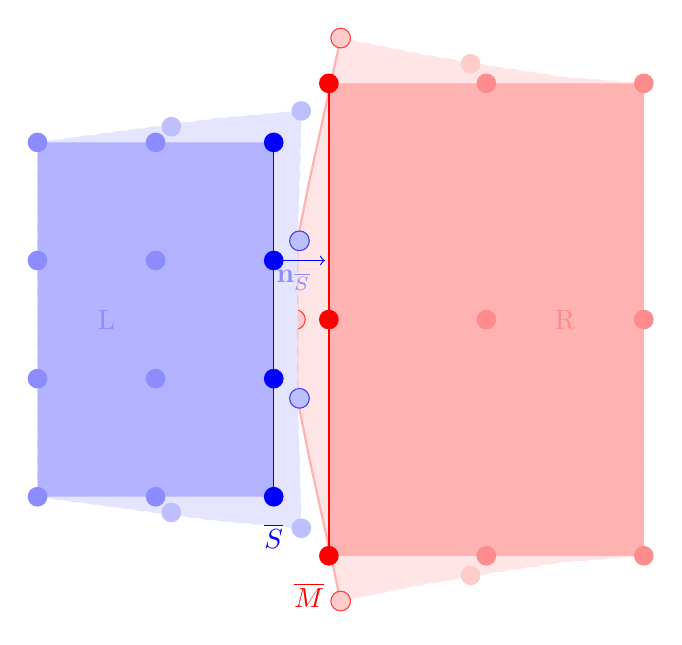
\begin{tikzpicture}
  % Master
  \begin{scope}[xshift=0.35cm]
    % Displaced
    \filldraw[red!10,dashed,opacity=10] plot [smooth]
    (4.0,-3.0) -- (4.0,3.0) --
    (3.0,3.075) -- (2.0,3.225) -- (1.0cm,3.400cm) -- (0.15cm,3.575cm) --
    (-0.25cm,1.75cm) -- (-0.40cm,1.0cm) -- (-0.40cm,-1.0cm) -- (-0.25cm,-1.75cm) --
    (0.15cm,-3.575cm) -- (1.0cm,-3.400cm) -- (2.0,-3.225) -- (3.0,-3.075) --
    cycle;
    \draw[thick,red!30] plot [smooth] (0.15cm,3.575cm) --(-0.25cm,1.75cm) -- (-0.40cm,1.0cm) -- (-0.40cm,-1.0cm) -- (-0.25cm,-1.75cm) -- (0.15cm,-3.575cm);
    \fill[red!20] ( 1.800cm, 3.250cm) circle (0.125);
    \fill[red!20] ( 0.150cm, 3.575cm) circle (0.125);    \draw[red!75] ( 0.150cm, 3.575cm) circle (0.125);
    \fill[red!20] (-0.425cm, 0.000cm) circle (0.125);    \draw[red!75] (-0.425cm, 0.000cm) circle (0.125);
    \fill[red!20] ( 0.150cm,-3.575cm) circle (0.125);    \draw[red!75] ( 0.150cm,-3.575cm) circle (0.125);
    \fill[red!20] ( 1.800cm,-3.250cm) circle (0.125);
    % Undisplaced
    \fill[thick,red!30,opacity=20] (0cm,3.0cm) -- (0,-3.0) -- (4.0,-3.0) -- (4.0,3.0) -- cycle;
    \draw[thick,red] (0cm,3.0cm) -- (0,-3.0);
    \begin{scope}
      \fill[red] (0cm, 3.0cm) circle (0.125);
      \fill[red] (0cm, 0.0cm) circle (0.125);
      \fill[red] (0cm,-3.0cm) circle (0.125);
    \end{scope}
    \begin{scope}[xshift=2.0cm]
      \fill[red!45] (0cm, 3.0cm) circle (0.125);
      \fill[red!45] (0cm, 0.0cm) circle (0.125);
      \fill[red!45] (0cm,-3.0cm) circle (0.125);
    \end{scope}
    \begin{scope}[xshift=4.0cm]
      \fill[red!45] (0cm, 3.0cm) circle (0.125);
      \fill[red!45] (0cm, 0.0cm) circle (0.125);
      \fill[red!45] (0cm,-3.0cm) circle (0.125);
    \end{scope}
    \node[red] at (-0.25cm,-3.50cm) {$\overline M$};
    \node[red!45] at  (3.0cm,0.0cm) {R};
  \end{scope}
  % Slave
  \begin{scope}[xshift=-0.35cm]
    % Displaced
    \filldraw[blue!10,dashed,opacity=10] plot [smooth]
    (-3.0,-2.25) -- (-3.0,2.25) --
    (-1.5,2.45) -- (-0.75,2.55) -- (0.35cm,2.65cm) --
    (0.325,1.75) -- (0.30,1.0) -- (0.30,-1.0) -- (0.325,-1.75) --
    (0.35,-2.65) -- (-0.75,-2.55) -- (-1.5,-2.45) --
    cycle;
    \fill[blue!25] (-1.30,  2.45) circle (0.125);
    \fill[blue!25] ( 0.35,  2.65) circle (0.125);
    \fill[blue!25] ( 0.327, 1.00) circle (0.125); \draw[blue!75] ( 0.327, 1.00) circle (0.125);
    \fill[blue!25] ( 0.327,-1.00) circle (0.125); \draw[blue!75] ( 0.327,-1.00) circle (0.125);
    \fill[blue!25] (-1.30, -2.45) circle (0.125);
    \fill[blue!25] ( 0.35, -2.65) circle (0.125);
    % Undisplaced
    \fill[thick,blue!30,opacity=20] (0cm,2.25cm) -- (0,-2.25) -- (-3.0,-2.25) -- (-3.0,2.25) -- cycle;
    \draw[blue] (0cm,2.25cm) -- (0,-2.25);
    \begin{scope}
      \draw[blue,->] (0cm,0.75cm) -- (0.65cm,0.75);
      \node[blue!45] at (0.25cm,0.5cm) {$\vecn_{\overline S}$};
      \fill[blue] (0cm, 2.25cm) circle (0.125);
      \fill[blue] (0cm, 0.75cm) circle (0.125);
      \fill[blue] (0cm,-0.75cm) circle (0.125);
      \fill[blue] (0cm,-2.25cm) circle (0.125);
    \end{scope}
    \begin{scope}[xshift=-1.5cm]
      \fill[blue!45] (0cm, 2.25cm) circle (0.125);
      \fill[blue!45] (0cm, 0.75cm) circle (0.125);
      \fill[blue!45] (0cm,-0.75cm) circle (0.125);
      \fill[blue!45] (0cm,-2.25cm) circle (0.125);
    \end{scope}
    \begin{scope}[xshift=-3.0cm]
      \fill[blue!45] (0cm, 2.25cm) circle (0.125);
      \fill[blue!45] (0cm, 0.75cm) circle (0.125);
      \fill[blue!45] (0cm,-0.75cm) circle (0.125);
      \fill[blue!45] (0cm,-2.25cm) circle (0.125);
    \end{scope}
    \node[blue!45] at  (-2.125cm,0.0cm) {L};
    \node[blue] at  (-0.0 cm, -2.75cm) {$\overline{S}$};
  \end{scope}
\end{tikzpicture}
\caption{Slave nodes
({\textcolor{blue}{$\overline S$}})
and master nodes ({\textcolor{red}{$\overline M$}}) on the corresponding surfaces.
Node coordinates are $x_{\overline S}$ and $x_{\overline M}$, respectively,
 while $u_{\overline S}$ and $u_{\overline M}$ are the corresponding displacements.
Lagrange multipliers $\lambda$ are colocated with the slave displacements $u_{\overline S}$ and prevent the penetration of $x_{\overline S} + u_{\overline S}$ (light blue) past $x_{\overline M} + u_{\overline M}$ (light red).
Nodes ({\textcolor{blue}S}) and ({\textcolor{red}M}) are those slave, correspondingly, master, nodes that are in contact.
Left ({\textcolor{blue}L}) and right ({\textcolor{red} R}) nodes only couple to {\textcolor{blue}S} and {\textcolor{red}M} elastically and include the {\textcolor{blue}{$\overline S$}} or, respectively,
{\textcolor{red}{$\overline M$}} nodes not in contact.
Observe that only the Lagrange multipliers (forces of constraint) corresponding to the slave nodes in contact (circled) are nonzero; the corresponding equations couple the slave nodes in contact to the master nodes (circled) adjacent
to the master boundary elements (dark displaced curvilinear edges) supporting the slave nodes in contact.
\label{fig:contact}
}
\end{figure}
\end{document}